% Created 2023-09-30 sáb 14:31
% Intended LaTeX compiler: pdflatex
\documentclass[11pt]{article}
\usepackage[utf8]{inputenc}
\usepackage[T1]{fontenc}
\usepackage{graphicx}
\usepackage{grffile}
\usepackage{longtable}
\usepackage{wrapfig}
\usepackage{rotating}
\usepackage[normalem]{ulem}
\usepackage{amsmath}
\usepackage{textcomp}
\usepackage{amssymb}
\usepackage{capt-of}
\usepackage{hyperref}
\usepackage{../modern}
\bibliography{../sample.bib}
\raggedbottom
\setcounter{secnumdepth}{2}
\author{Luis Eduardo Galindo Amaya (1274895)}
\date{18 de Septiembre 2023}
\title{Instalación, configuración y administración de un servidor Linux}
\hypersetup{
 pdfauthor={Luis Eduardo Galindo Amaya (1274895)},
 pdftitle={Instalación, configuración y administración de un servidor Linux},
 pdfkeywords={},
 pdfsubject={},
 pdfcreator={Emacs 27.1 (Org mode 9.3)}, 
 pdflang={Spanish}}
\begin{document}

\modentitlepage{../images/escudo-uabc-2022-1-tinta-pos.png}
\tableofcontents
\pagebreak
\datasection{Individual}

\section{Introduccion}
\label{sec:org4ee9eda}
La noticia que encontre en linux fue la siguiente: \\
Habla de un error encontrado en el kernel de Linux se refiere a una 
vulnerabilidad de seguridad identificada como CVE-2023-32233 que permite a 
usuarios autenticados localmente obtener derechos adicionales en el sistema, 
incluidos privilegios de root. Piotr Krysiuk fue le responsable de eonctrar 
esta vulnerabilidad, probablemente será parcehada en unos dias.

\section{Instaslacion de Linux}
\label{sec:orgf41260e}
\subsection{Creacion de la maquina virtual}
\label{sec:orgdf49aa6}
\begin{figure}[htbp]
\centering
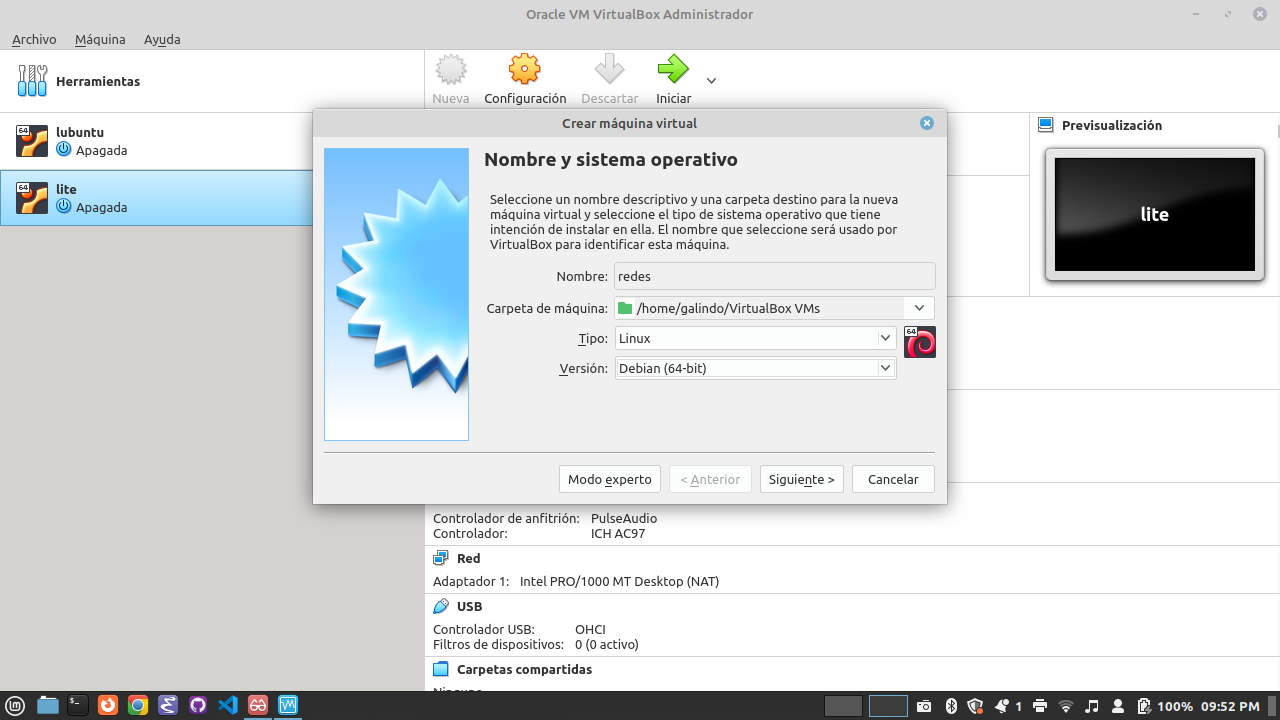
\includegraphics[width=9cm]{img/Captura de pantalla de 2023-09-17 21-52-24.png}
\caption{Utilizando VirtualBox}
\end{figure}

\pagebreak

\subsection{Arrancado el ISO}
\label{sec:org96bfe3f}
\begin{figure}[htbp]
\centering
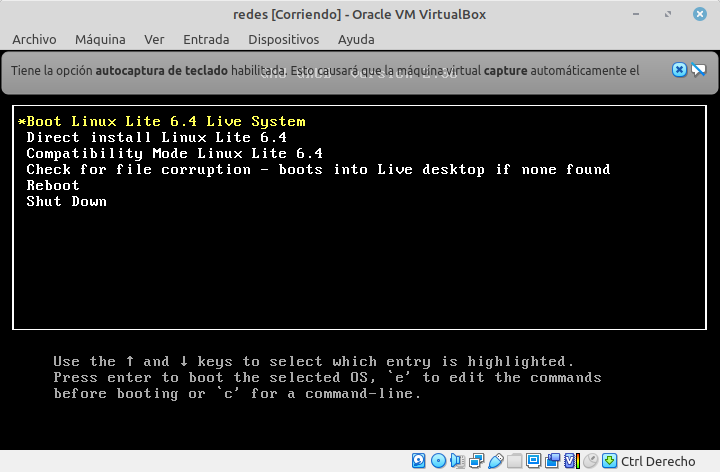
\includegraphics[width=10cm]{img/Captura de pantalla de 2023-09-17 21-54-09.png}
\caption{Pantalla de boot}
\end{figure}

\subsection{Instalando los programas y actualizaciones}
\label{sec:org8be8722}
\begin{figure}[htbp]
\centering
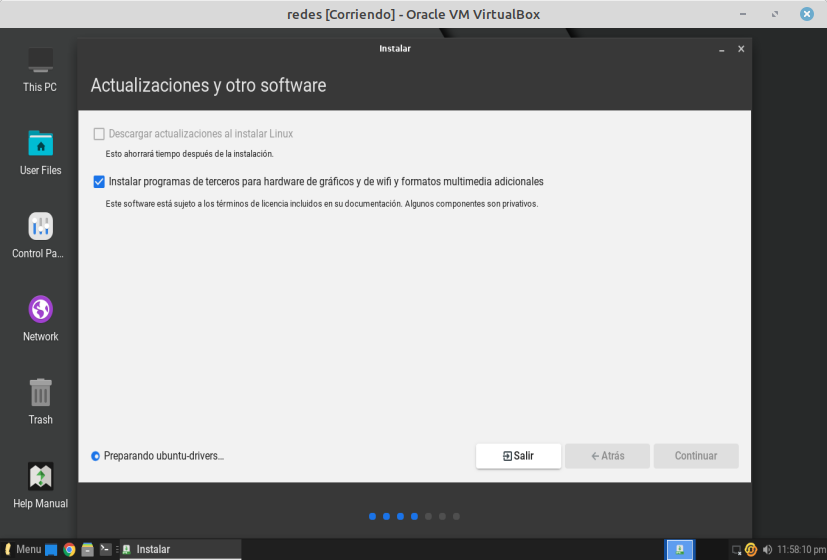
\includegraphics[width=10cm]{img/Captura de pantalla de 2023-09-17 21-58-10.png}
\caption{Instalación de linuxLite}
\end{figure}

\pagebreak

\subsection{Lista de usuarios}
\label{sec:orge508fa1}
\begin{figure}[htbp]
\centering
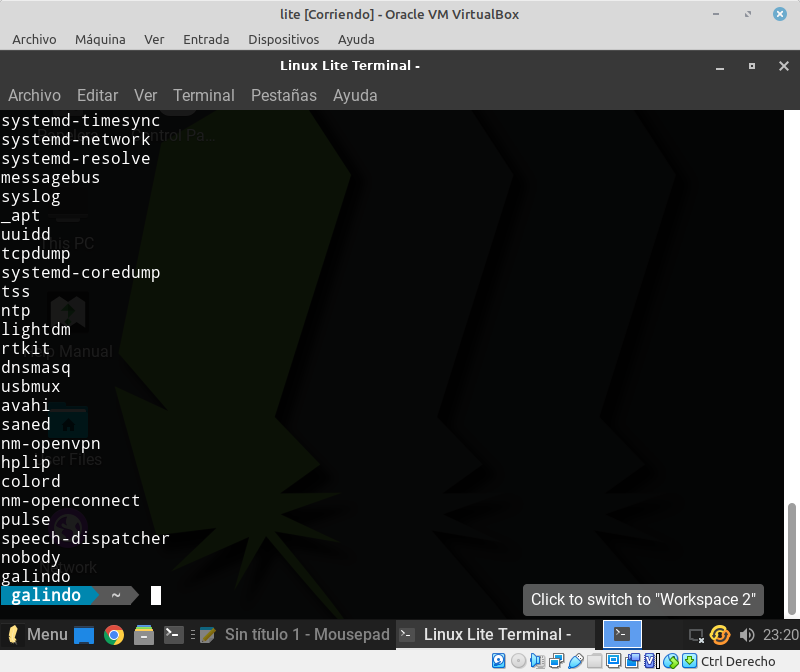
\includegraphics[width=9cm]{img/usuarios.png}
\caption{Usarios hasta el momento}
\end{figure}

\subsection{Creando usuarios}
\label{sec:org5e9f2f9}
\begin{figure}[htbp]
\centering
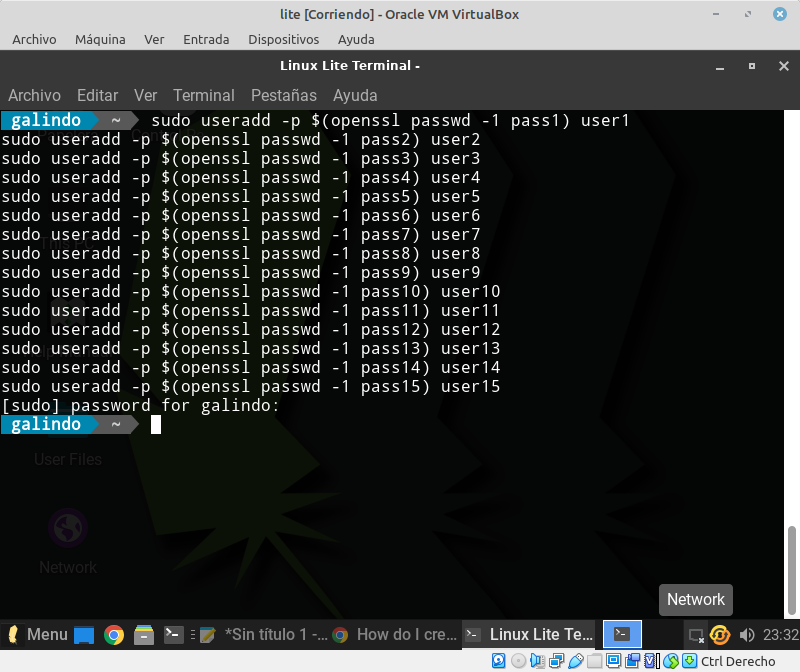
\includegraphics[width=9cm]{img/Captura de pantalla de 2023-09-17 23-32-10.png}
\caption{Utilizando comandos para crear Usuarios}
\end{figure}

\pagebreak

\subsection{Listar usuarios}
\label{sec:org3f1105d}
\begin{figure}[htbp]
\centering
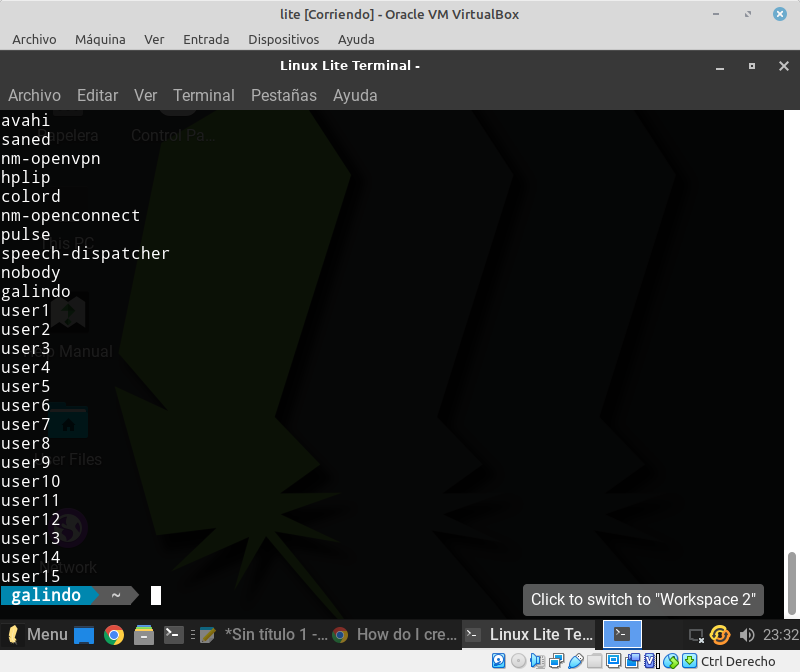
\includegraphics[width=10cm]{img/Captura de pantalla de 2023-09-17 23-32-29.png}
\caption{Lista de suaurios}
\end{figure}

\section{Conclusión}
\label{sec:org21c5978}
A lo largo de la practica aprendi como crear usuarios y como 
instalar uan distribusion linux. Como ingenierios en software pienso que debemos 
aprender a trabajar con diversos sistemas operativos.
\end{document}
